\documentclass{article}
\usepackage[utf8]{inputenc}
\usepackage{hyperref}

\title{Übung 4}
\author{Laurenz Weixlbaumer, 11804751}
\date{November 2018}

\renewcommand\thesubsection{(\alph{subsection})}

\usepackage{enumitem}
\usepackage{mathtools}

\begin{document}

\maketitle

\section{Zusammensetzung und Testung der ALU}

\begin{enumerate}[label=(\alph*)]

\item Schaltbild der ALU.

\begin{figure}[htp]
\begin{center}
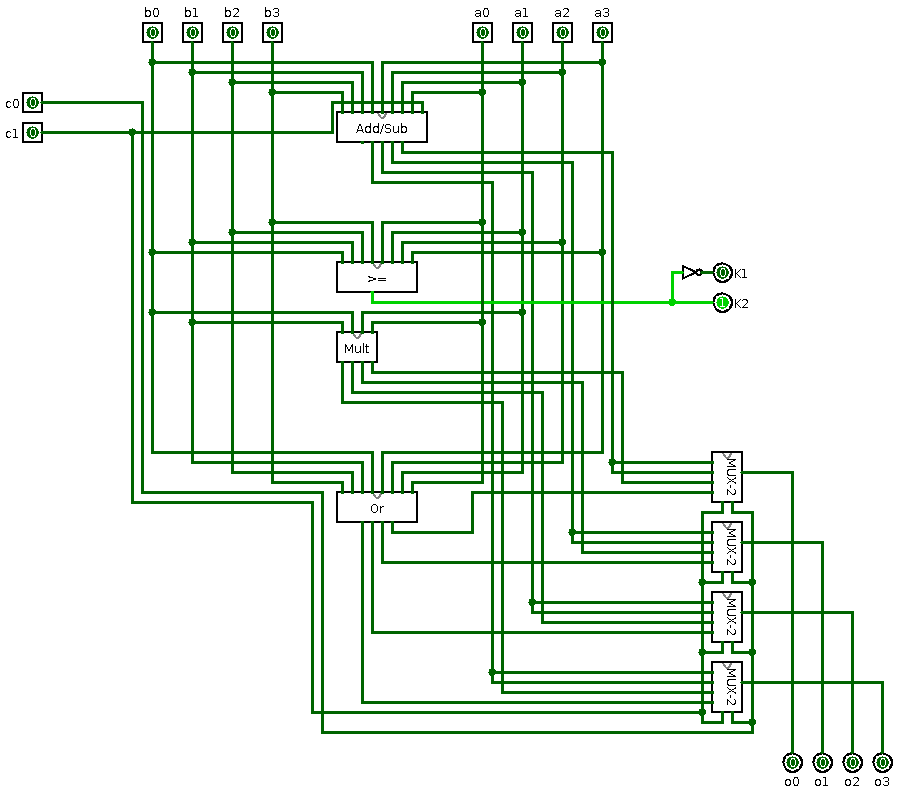
\includegraphics[width=14cm]{alu_circuit.png}
\end{center}
\end{figure}

\item Testung der ALU.

\begin{description}

\item [$1110_2$ + $0111_2$, Ansteuerung: $00_2$]

\begin{figure}[htp]
\begin{center}
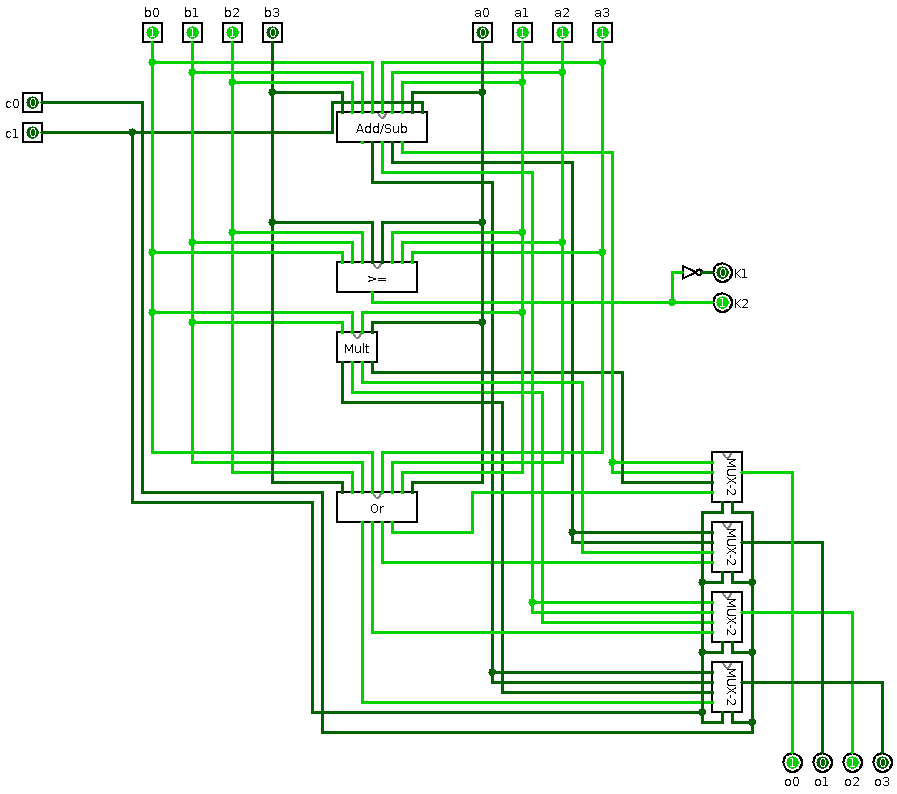
\includegraphics[width=14cm]{alu_circuit_00_marked.png}
\end{center}
\end{figure}

\clearpage

\item [$1111_2 - 1110_2$, Ansteuerung: $01_2$]

\begin{figure}[htp]
\begin{center}
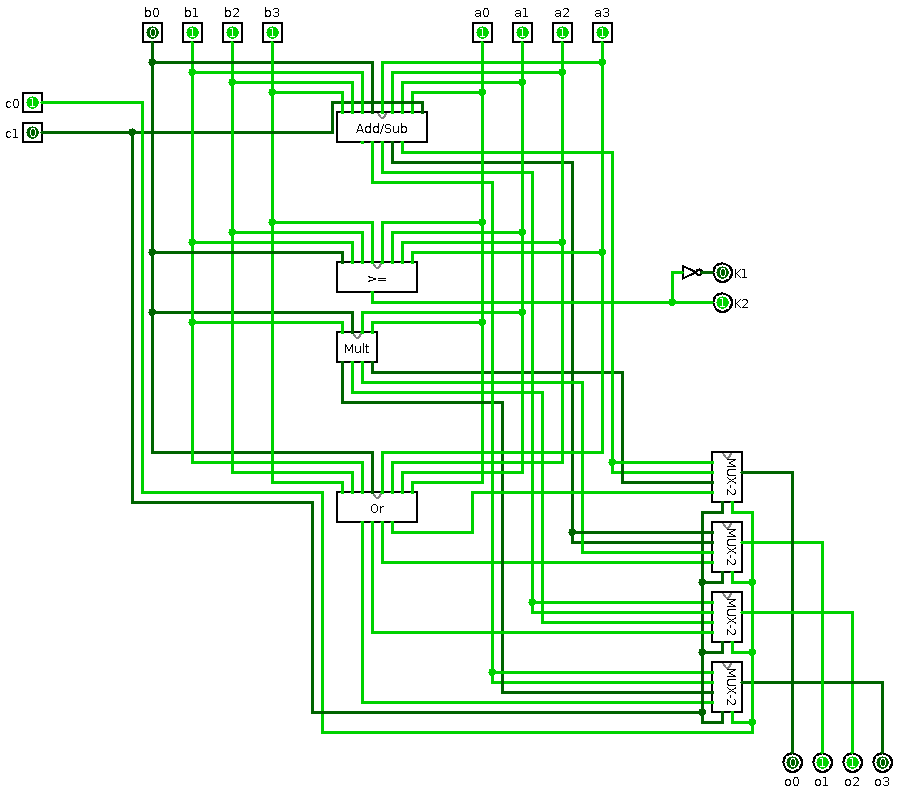
\includegraphics[width=14cm]{alu_circuit_01_marked.png}
\end{center}
\end{figure}

\clearpage

\item [$1010_2 * 1101_2$, Ansteuerung: $10_2$]

\begin{figure}[htp]
\begin{center}
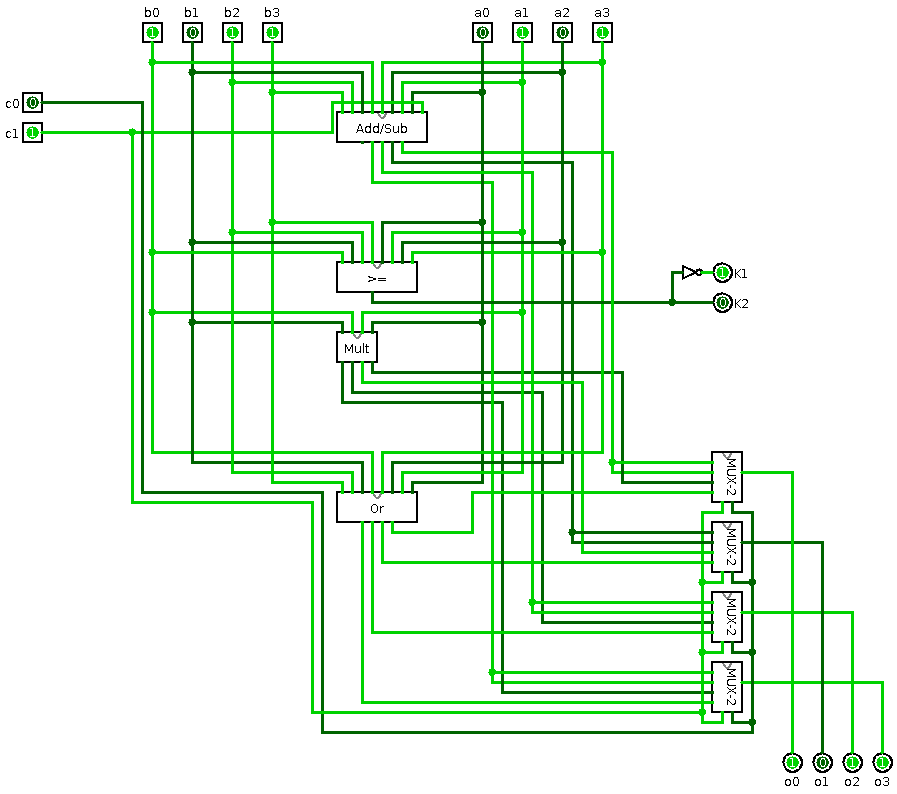
\includegraphics[width=14cm]{alu_circuit_10_marked.png}
\end{center}
\end{figure}

\clearpage

\item [$1010_2 \lor 1110_2$, Ansteuerung: $11_2$]

\begin{figure}[htp]
\begin{center}
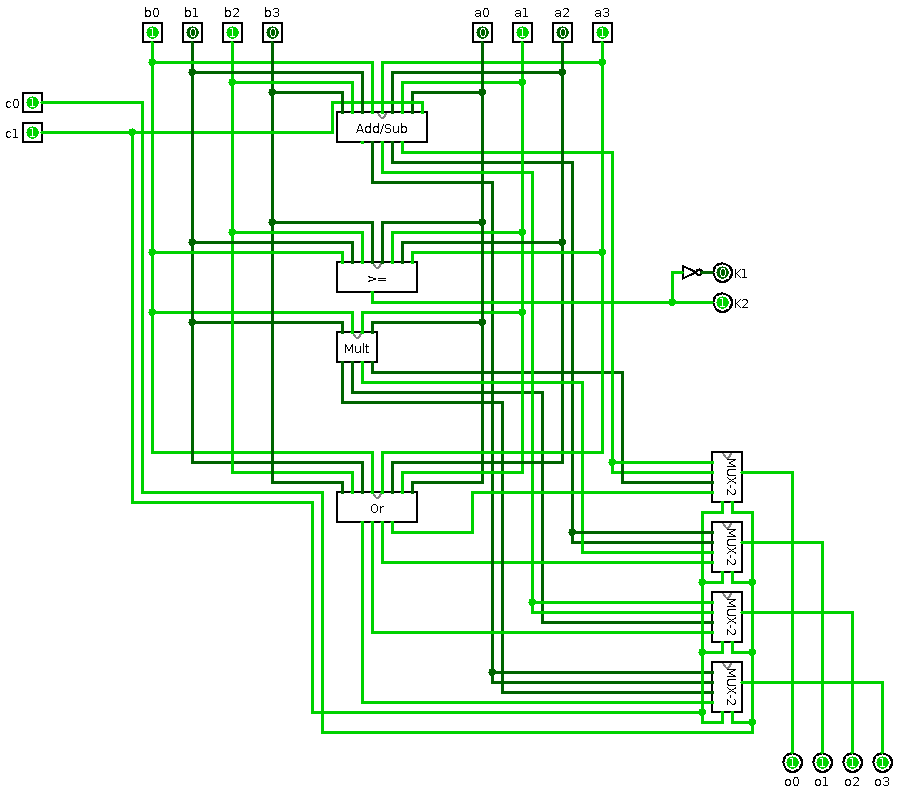
\includegraphics[width=14cm]{alu_circuit_11_marked.png}
\end{center}
\end{figure}

\end{description}

\end{enumerate}

\end{document}
